% \begin{figure*}[htbp]
% \centering
% \resizebox{\textwidth}{!}{%
% \begin{tikzpicture}[
%     node distance=1.5cm and 2cm, % lebih rapat
%     process/.style={rectangle, draw=black, thick, minimum width=2.2cm, minimum height=0.8cm, font=\small},
%     data/.style={trapezium, draw=black, thick, trapezium left angle=70, trapezium right angle=110, minimum width=2cm, minimum height=0.8cm, font=\small},
%     decision/.style={diamond, draw=black, thick, minimum width=2cm, minimum height=1cm, font=\small},
%     arrow/.style={->, thick}
% ]

% % Row 1: Data Processing
% \node[data, fill=inputcolor] (raw) {Raw Dataset};
% \node[process, fill=processcolor, right=of raw] (eng) {Feature\\Engineering};
% \node[process, fill=processcolor, right=of eng] (norm) {Normalization};
% \node[process, fill=processcolor, right=of norm] (window) {Windowing};

% % Row 2: Model
% \node[process, fill=tcncolor, below=1.5cm of window] (tcn) {Stochastic\\TCN};
% \node[process, fill=tcncolor, left=of tcn] (mc) {MC Dropout\\Inference};
% \node[data, left=of mc] (pred) {Predictions\\+ Uncertainty};

% % Row 3: Anomaly Detection
% \node[process, fill=anomalycolor, below=1.5cm of mc, xshift=-6.4cm] (error) {Error\\Calculation};
% \node[decision, fill=anomalycolor, right=of error] (thresh) {Threshold\\Check};
% \node[data, right=of thresh] (anomaly) {Anomaly\\Flags};

% % Connections
% \draw[arrow] (raw) -- (eng);
% \draw[arrow] (eng) -- (norm);
% \draw[arrow] (norm) -- (window);
% \draw[arrow] (window) -- (tcn);
% \draw[arrow] (tcn) -- (mc);
% \draw[arrow] (mc) -- (pred);
% \draw[arrow] (pred) -- (error);
% \draw[arrow] (error) -- (thresh);
% \draw[arrow] (thresh) -- (anomaly);

% % Feedback loop
% \draw[arrow, dashed, gray] (anomaly.north) -- ++(0,1) -| (tcn.south);

% \end{tikzpicture}%
% }
% \caption{End-to-End Stochastic TCN Anomaly Detection workflow}
% \label{fig:STCN_workflow}
% \end{figure*}

\begin{figure*}[!t]
    \centering
    % Make sure you have \usepackage{graphicx} in your preamble
    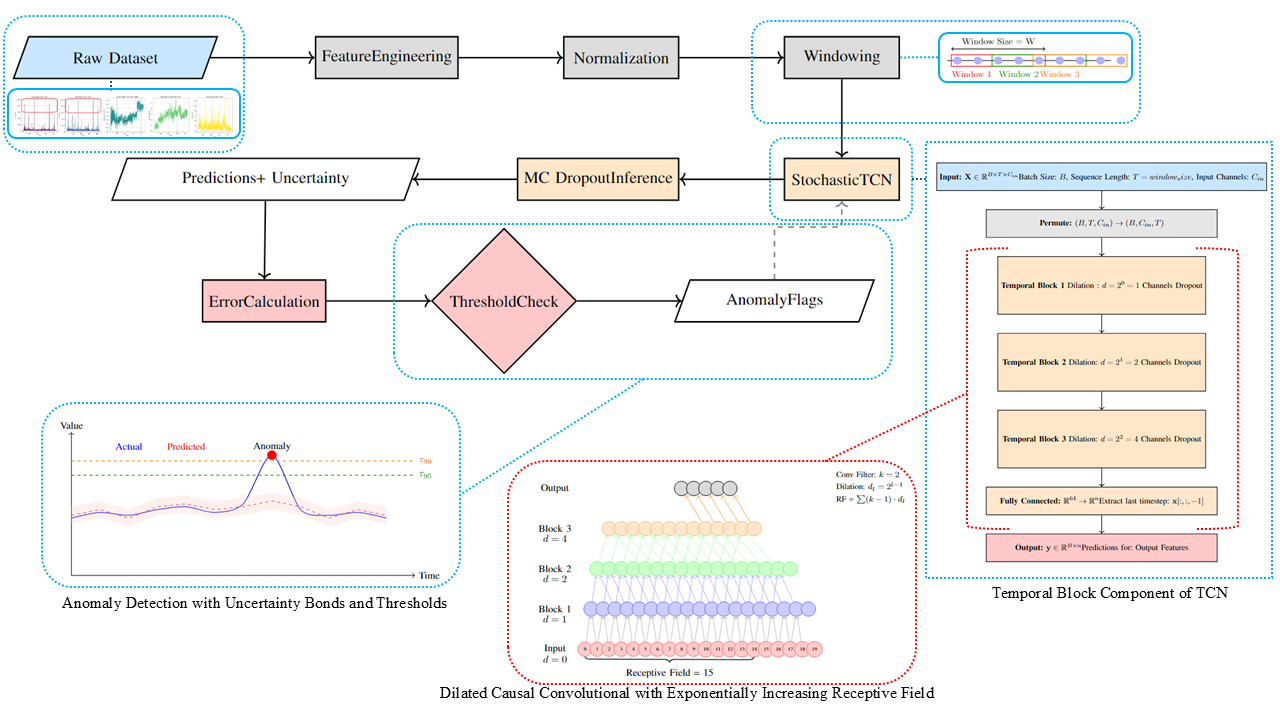
\includegraphics[width=\textwidth]{images/End to End Stochastic Workflow.png}
    \caption{End to End Stochastic TCN Anomaly Detection Workflow.}
    \label{fig:STCN_workflow}
\end{figure*}